\chapter{Materials and Methods}
\label{chap:final-methods}

\section{Data, curation and traceability}
\subsection{\acrshort{ctmar} Dataset and Reference Sources}

The main dataset used in this work comes from the\acrfull{ctmar} \cite{hanedaAAPMCTMetal2025, AAPMCTMARBenchmarkTool} promoted by the\acrfull{aapm} and consists of 14,000 training pairs containing\acrshort{ct} images with simulated metal artifacts and their original artifact-free versions. The data was generated through a hybrid simulation framework \cite{petersHybridTrainingDatabase2025}, which incorporates publicly available clinical images and simulated metallic objects with the CatSim simulator, integrated into the open-source XCIST toolkit \cite{wuXCISTOpenAccess2022}. The dataset is distributed into two anatomical categories:

\begin{itemize}
    \item \textbf{Head}: 1.626 (11.61\%) samples derived from the \textit{UCLH Stroke EIT Data} \cite{gorenMultifrequencyElectricalImpedance2018, gorenUCLHStrokeEIT2017};
    \item \textbf{Body}: 12.374 (88.38\%) samples derived from the \textit{NIH DeepLesion Data} \cite{yanDeepLesionAutomatedMining2018}.
\end{itemize}

Where the folders in the \textit{body} category contained trunk\acrshort{ct}s, covering axial, thoracic, and abdominal slices. The data is organized into subfolders, each containing up to 1,000 samples. Only the following files were used for training and validation:

\begin{enumerate}
    \item \textbf{Metal-Free images (reference):} Files contained in the \textit{Target} folder of size 512×512×1 pixels;
    \item \textbf{Images with metal artifacts (corrupted):} Files contained in the \textit{Baseline} folder of size 512×512×1 pixels.
\end{enumerate}

All image files (.raw) in the dataset are presented in binary format without a header, with float32 precision in little-endian order. The images were already converted from linear attenuation coefficients (in mm$^{-1}$ units) to\Acrfull{hu}, using the normalization value of 0.02 mm$^{-1}$ for water.
There was not additional information about which exam each slice belonged to, if they were from the same patient, or which specific anatomical regions were represented. The only available information was the organization by folder, indicating the anatomical category (Head or Body). The lack of detailed metadata imposed the need for a careful pre-processing approach to ensure that the data was properly organized and used during model training and validation. Therefore, a significant effort was dedicated to tracking the images to the original datasets (UCLH Stroke EIT Data and NIH DeepLesion Data) to obtain additional information about the exams and patients, allowing for an appropriate partitioning of the data.

\subsection{Partitioning at patient level}

The data partitioning was stratified by patients, ensuring that slices from the same patient were not distributed across training, validation, and test sets. This approach prevents information leakage and ensures a more realistic assessment of the models generalization capability.

%________________________________________________________________________________________________________________________________________________________________

Due to the lack of detailed clinical metadata in the\acrshort{ctmar} dataset, an algorithmic screening of the slices to the original datasets (UCLH Stroke EIT and NIH DeepLesion Data) was necessary to enable the association of the provided metadata with the\acrshort{ctmar} slices. This process allowed for the identification of which exam and patient from DeepLesion/UCLH Stroke EIT each\acrshort{ctmar} image belonged to. This information was subsequently used to perform patient-level partitioning of the data into training, validation, and test sets, reducing the risk of data leakage between experimental sets.


The correct separation of the data is particularly important in medical imaging studies based on\acrshort{dl}, once slices belonging to the same exam often present high anatomical similarity. Thus, the simultaneous presence of images from the same patient in training and testing can artificially inflate the model's performance and compromise the assessment of its generalization capability \cite{onerTrainingMachineLearning2020}. 

The Deep Lesion images \cite{yanDeepLesionAutomatedMining2018} are stored in 16-bit PNG format, while the\acrshort{ctmar} images are provided in .raw format directly in\acrshort{hu}. The UCLH Stroke EIT \cite{gorenMultifrequencyElectricalImpedance2018} provides the exams in DICOM format. Therefore, regardless of the original format, all images were converted to\acrshort{hu} before comparison, ensuring uniformity across the different datasets.

After the conversion, all images was represented on the same intensity scale to allow direct comparison.

The screening algorithm was based on fact that\acrshort{ct} images preserve quantitative information in\acrshort{hu}, which directly reflects the tissue attenuation properties. Since anatomical structures exhibit high spatial continuity between consecutive slices of the same aquisition, images correponding to the same anatomical slice tend to present similar\acrshort{hu} distributions and highly consistent global structural patterns \cite{zhouwangImageQualityAssessment2004, hsiehComputedTomographyPrinciples2009}.   

That way, the method was not designing to verify absolute pixel-to-pixel equality between images, but rather to determine whether the overall structural organization of the anatomy remains extremely similar across different representations of the same slice. This behavior is particularly important because small local variations in intensity, numerical discretization, and linear transformations associated with storing format conversion tend to preserve the global anatomical structure of the image even when small local intensity variations occur \cite{zhouwangImageQualityAssessment2004,hsiehComputedTomographyPrinciples2009}.

Thus, the adopted methodology seeks to identify correspondences between images based on global structural similarity, allowing for a margin of local variation that does not compromise the correct identification of the exam and patient of origin. Initially, each image was reduced to a campact representation through \textit{downsampling}, preserving mainly the relevant global anatomical information. This step significantly reduces the computational cost without compromising the overall structure of the image.

Subsequently, a representative vector (\textit{fingerprint}) was calculated for each image. The fingerprints of the\acrshort{ctmar} images were then compared with the fingerprints of the DeepLesion and UCLH Stroke EIT images using a normalized dot product-based vector similarity metric (cosine similarity). It was chosen for being invariant to global scale differences between vectors — a relevant property given that the images come from different formats with different intensity normalizations. For each\acrshort{ctmar} image, the image with the highest similarity score was selected.

Since the majority of the\acrshort{ctmar} images originated from DeepLesion, the screening process was initially prioritized on that dataset. Subsequently, the same methodology was applied to the DICOM exams from UCLH Stroke EIT to identify the remaining images. In this way, it was possible to implement a unified traceability strategy regardless of the storage format of the original datasets.

The matching was considerd valid only when the score of similarity exceeded a previously defined empirically threshold. Cases with very high scores were automatically marked as safe matches, as it was observed that all pairs visually analyzed with a score above 0.993 effectively corresponded to the same image. To maintain an additional safety margin, the match was considered automatically valid only when the score exceeded 0.994.

Scores below this threshold indicated potentially ambiguous matches and were subjected to manual visual inspection. Scores below approximately 0.98 indicated clearly incorrect matches and were automatically discarded without the need for manual review. Thus, all pairs with scores between 0.98 and 0.994 were visually analyzed to confirm the validity of the match. In order to avoid unnecessary exclusion of pairs, all pairs with a score below 0.98 for both datasets (DeepLesion and UCLH Stroke EIT) were subjected to visual inspection to ensure they were not erroneously discarded.

For the 530 pairs that remained without approved matches after direct search in both source datasets, a complementary indirect matching step was applied. In this step, each unmatched\acrshort{ctmar} image was compared with already traced\acrshort{ctmar} images. The most similar neighbors were used to select candidate exams from DeepLesion and then all \textit{slices} of those exams were searched with $64\times64$ dimension \textit{fingerprints}. The 530 proposals were visually inspected: 95 matches were approved and incorporated into the consolidated manifest, while 435 remained without a safe match and were excluded.

Moreover, the algorithm was designed to automatically ignore images that had already been verified as correct matches, reducing redundancies and accelerating future reprocessing. Given the high number of images present in the datasets, the processing was parallelized and optimized through the use of vectorized matrix operations. When available, the algorithm utilizes\acrshort{gpu} acceleration to reduce execution time. The calculated fingerprints were also cached to avoid unnecessary recomputation in subsequent runs.

Although, the compact representation based exclusively on the mean of block intensities\acrshort{hu} is efficient, it can theoretically generate false positives when different patients exams are acquired with identical acquisition protocols or present very similar anatomical structures. Since these conditions tend to produce similar intensity distributions and, consequently, fingerprints with high scores. To mitigate this risk, a conservative automatic acceptance threshold (0.994) was adopted and a systematic visual validation of all pairs with scores between 0.98 and 0.994 was performed. Additionally, as a complementary safeguard, all automatic matches were analyzed in terms of\acrshort{ms-ssim}, where the pairs with the most critical scores were subjected to an additional visual review to ensure the reliability of the matches.


Despite that, this limitation does not compromise the main objective of the methodology. Even though consecutive slices from the same exam often present high spatial redundancy and can therefore obtain very similar similarity scores. The purpose of the algorithm was not to perform rigorous voxel-to-voxel alignment, but rather to correctly identify the exam and patient of origin of each\acrshort{ctmar} image. In this way, even potential ambiguities between adjacent slices remain restricted to the same anatomical volume and do not introduce a relevant risk of data leakage between training, validation, and test sets. 

The literature demonstrates that the quality of the pairs used in supervised studies directly influences the performance and generalization capability of\acrshort{mar} models \cite{linDuDoNetDualDomain2019, kleberAdvancementsSupervisedDeep2024}. In addition, structural metrics of image quality, such as\acrshort{ssim}, have been widely used in medical imaging due to their higher sensitivity to structural preservation \cite{zhouwangImageQualityAssessment2004}. Although the implemented method does not directly use\acrshort{ssim}, the adopted strategy seeks to precisely preserve the global structural information of the image during the matching process.

Moreover, the data utilization without any screening treatment would condition the entire project to an inherent data leakage from the dataset, compromising the evaluation of the models performance and the validity of the results. Thus, even if the screening method is not perfect, it represents a significant improvement over the total absence of screening, ensuring a more reliable basis.

Taking this into account, this step constituted an important quality control procedure for the experimental dataset and was fundamental to ensure an appropriate partitioning of the data used in this work.

%___________________________________________________________________________________________________________________________

\subsection{Anatomical Distribution and Stratification}

Stratification was implemented within each subset (train/val/test) to maintain the anatomical proportion at the patient level, ensuring that the relative proportion between categories is preserved across all subsets. In this way, the anatomical balance is preserved, ensuring that the models are trained and evaluated on an appropriate representation of the anatomical diversity present in the original dataset.

The patient-level partition was defined only once, with a fixed random seed, maintaining approximately 70\% of the patients for training, 15\% for validation, and 15\% for testing. This fixed partition ensured independent subsets for validation and testing and was kept unchanged across all experimental repetitions.

The resulting anatomical and split distributions are presented in \autoref{subsec:results-anatomical-distribution}.
\section{Pre-processing}

\subsection{Integrity Verification}

All pairs were validated through an integrity report, which checks for the existence of both sides of the pair (artifact image and clean image). There were no pairs with missing data, ensuring that the dataset was complete and ready for subsequent pre-processing and model training steps.

\subsection{Background Removal through Body Mask}

The\acrshort{ct} images often contain large background areas that do not contribute to the task of metal artifact removal. That creates a class imbalance in the training data, where irrelevant background voxels dominate over the anatomical regions of interest. This imbalance, in turn, hinders the learning and deviates the model focus from clinically relevant structures \cite{taghanakiComboLossHandling2021, kesimalUseDeepLearning2026}. To address this challenge, a pre-processing step also based on\acrshort{dl} was implemented. A\acrshort{unet} was trained to segment the body tissue from the background, generating binary masks that were applied to the original images to isolate the regions of interest. This model was trained using $\sim$ 1,500 samples from the\acrshort{ctmar}, where the segmentation masks were automatically generated through a thresholding process. Additionally, a fraction of the generated masks was subjected to iterative manual refinement to improve data quality and was used to retrain the model. This process was repeated until masks of sufficient quality for the intended purpose were obtained.
This step was essential to reduce the influence of background artifacts and improve the quality of features extraction during training. 

\subsection{Intensity Window and Normalization}

The\acrshort{ctmar} source image intensities were expressed in \acrshort{hu}. A common intensity window of $[-1000, 400]\acrshort{hu}$ was applied to all images, followed by linear normalization to $[0,1]$. Each clean/artifact image pair was then independently resized using bicubic interpolation and stored as a single-channel two-dimensional tensor of $256 \times 256$ pixels.

\subsection{Artifact Mask for Auxiliary Supervision}
Binary difference masks of the affected regions by artifacts were produced and used as an additional supervision signal in the dual architeture. These masks are exclusively used during the training and are not required during inference. The binary difference mask is formally defined as: 
\begin{equation}
M_{diff}(i,j) = \begin{cases}
1 ; & \text{if } |I_{artifact}(i,j) - I_{clean}(i,j)| > \tau \\
0 ; & \text{otherwise}.
\end{cases}
\end{equation}
\noindent where $I_{artifact}$ represents the image with artifacts, $I_{clean}$ the clean reference image, and $\tau$ is the normalized difference threshold. The value of this threshold was empirically defined to capture regions with perceptible differences while maintaining robustness to low-amplitude noise.

\section{Compared Architectures}
\subsection{U-Net Single Supervision}

The first model consist of an architecture based on\acrshort{unet} \cite{ronnebergerUNetConvolutionalNetworks2015}, composed of encoder-decoder with skip connections. Li et al \cite{liUNetBasedDynamic2024}, apply blocks of\Acrfull{bn} and\acrfull{relu} activation functions after each dynamic convolution. This work does something similar, but chooses to use standard convolutions with $3\times3$ kernel, followed by\acrshort{bn} blocks and\acrshort{relu} activation functions. The choice for standard convolutions is justified by simplicity and computational efficiency, in addition to maintaining the approach used by Ronneberger et al \cite{ronnebergerUNetConvolutionalNetworks2015}. Like Li et al \cite{liUNetBasedDynamic2024}, the decoder also uses bilinear upsampling. This architecture has only one output.

\begin{figure}[htbp]
\centering
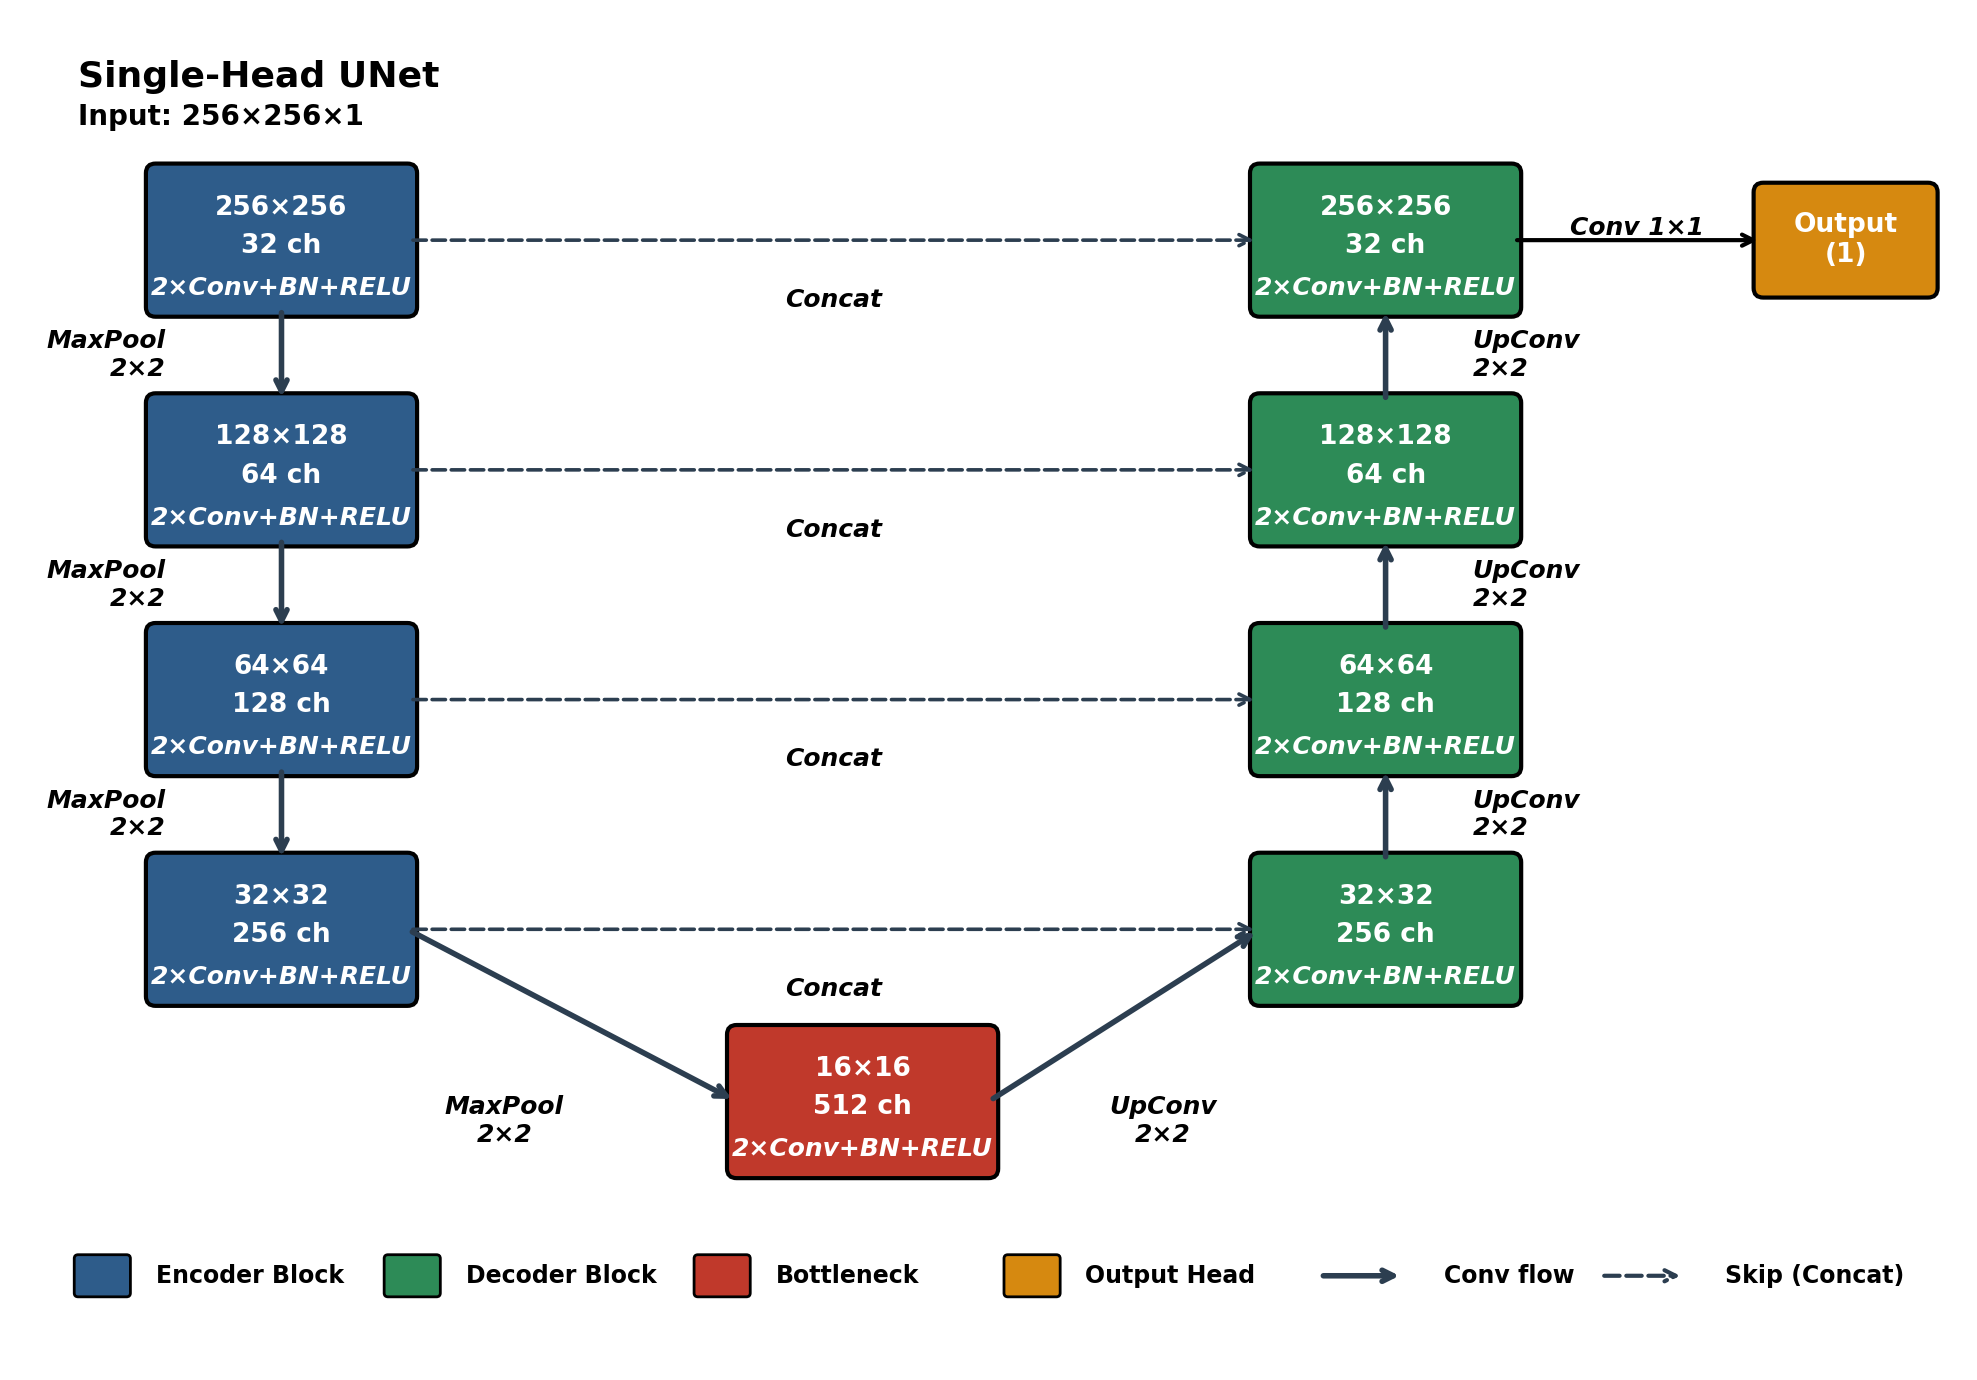
\includegraphics[width=0.95\linewidth]{Figures/Generated/materials/unet-single-compact-132d4a1a.png}
\caption[Single Supervision U-Net architecture]{Single supervision arquitecture diagram.}
\end{figure}

\subsection{U-Net Dual Supervision}

A variation of the model described above was conceived, maintaining the shared \textit{encoder} and \textit{decoder} and adding an independent output in the last layer. Thus, there are two distinct outputs in the decoder, each with its own loss function. The first output is responsible for reconstructing the corrected image, while the second output is dedicated to predicting the artifact mask.

The rationale for adding the auxiliary supervision of the artifact mask is based on the premise that the presence of an additional loss focused on segmenting regions affected by artifacts can provide complementary information to the model, aiding in learning more robust and discriminative representations. This approach is inspired by previous works that have shown that multi-task supervision can improve performance in related tasks \cite{caruanaMultitaskLearning, ruderOverviewMultiTaskLearning2017}.

The two architectures were evaluated against each other to determine the impact of the additional supervision with artifact mask on reconstruction quality and artifact reduction capability. All model bases are identical, with the presence of the artifact mask prediction output being the only difference in the second version. Thus, the comparison between the two architectures is fair and isolated, allowing for an exclusive evaluation of the impact of the additional supervision of the artifact mask.

\begin{figure}[htbp]
\centering
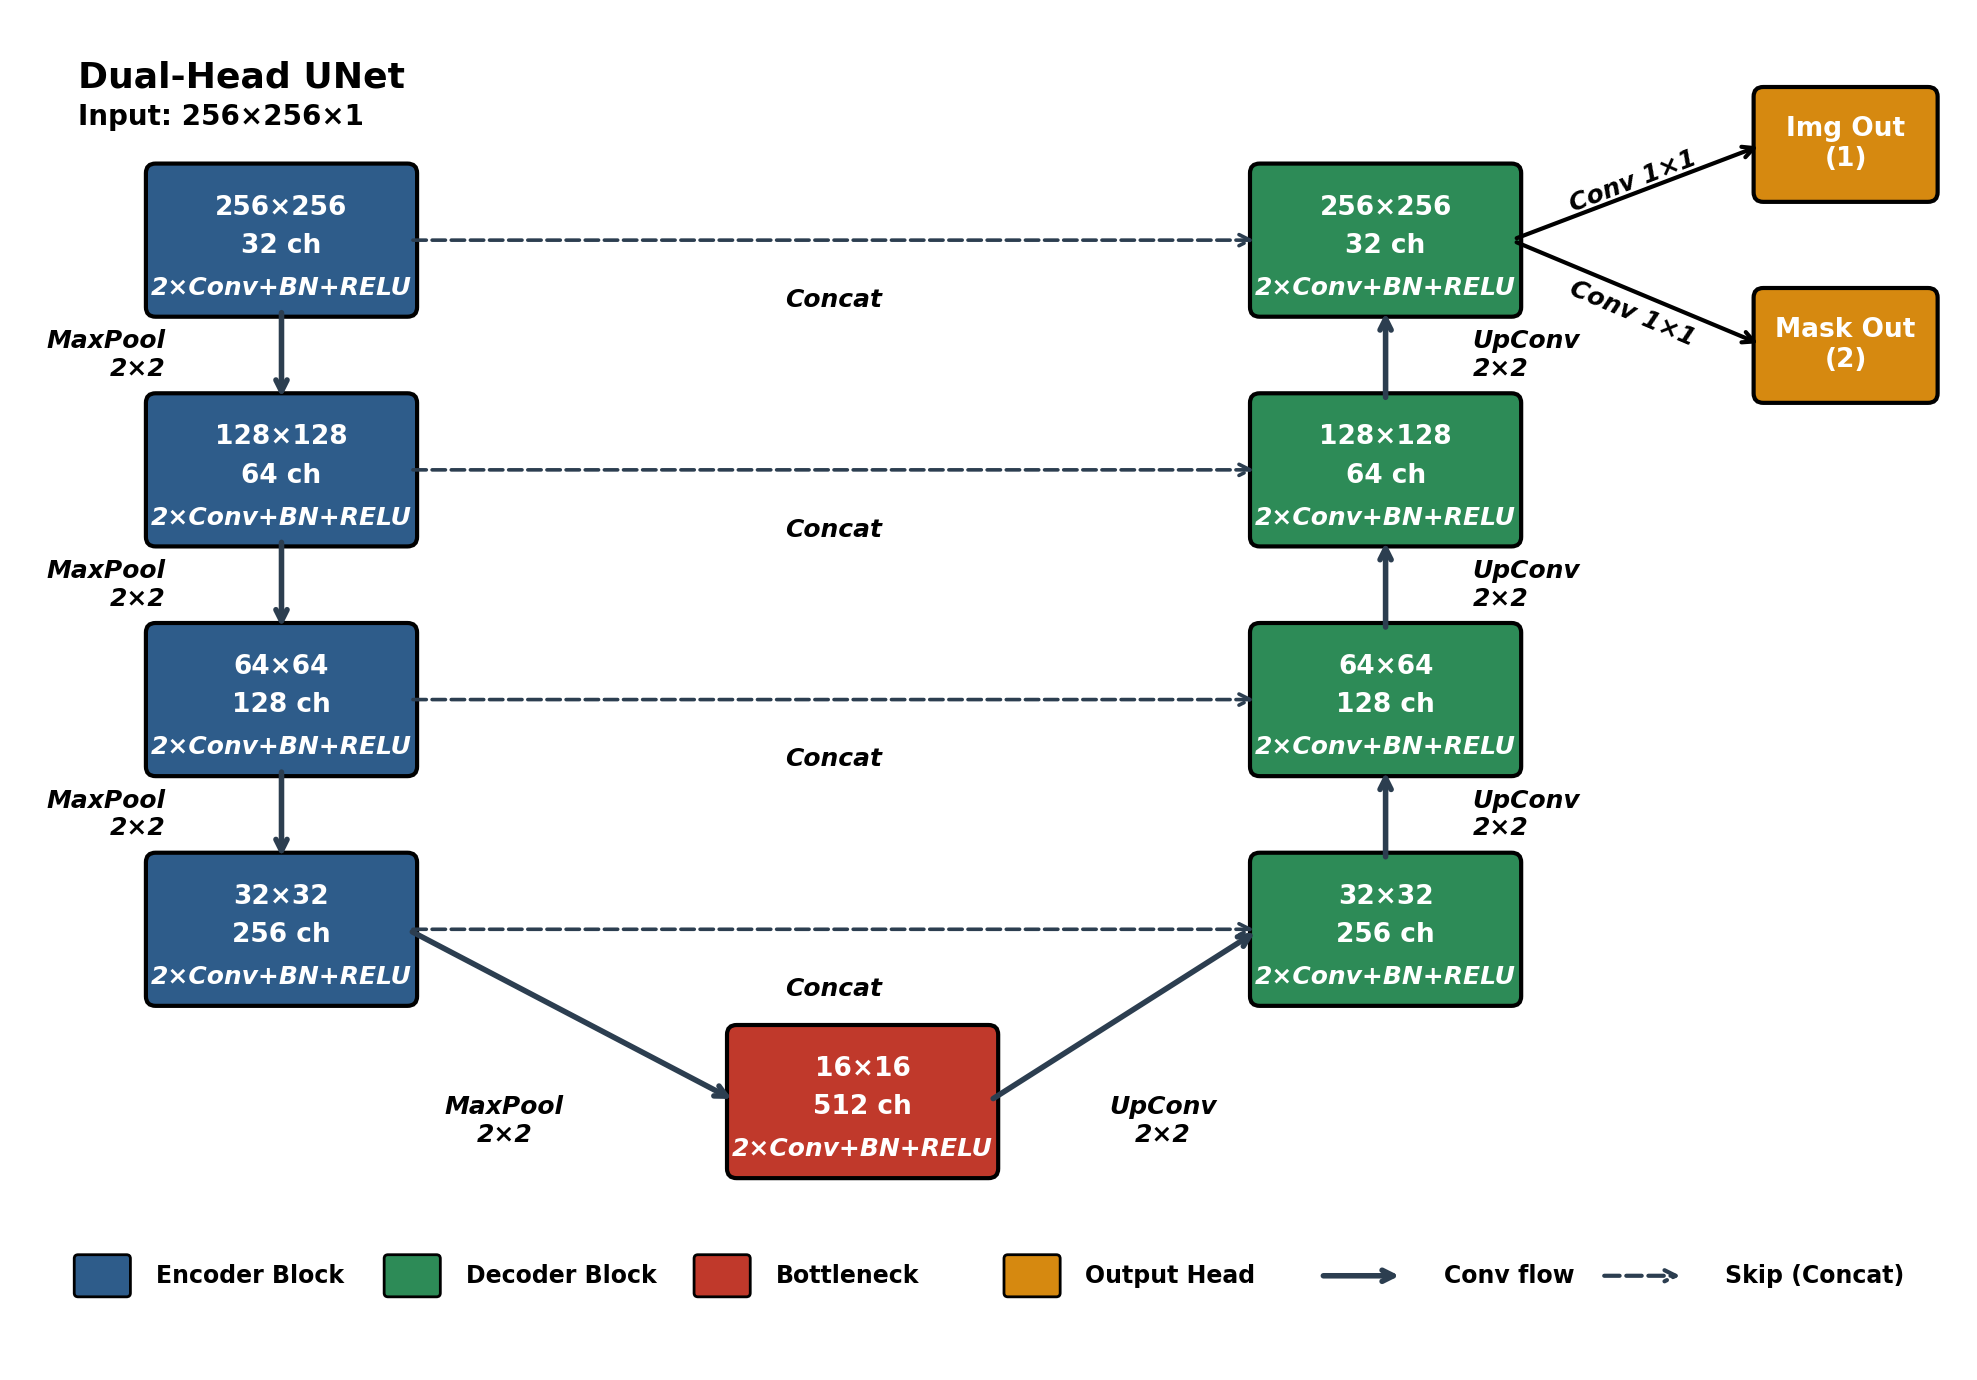
\includegraphics[width=0.95\linewidth]{Figures/Generated/materials/unet-dual-compact-8441faa2.png}
\caption[Dual Supervision U-Net architecture]{Dual supervision architecture diagram.}
\end{figure}

\section{Reproducible Training}

\subsection{Settings, determinism and two-stage selection}

Both models were trained under the same settings, with \textit{float32} precision. To assess stability against different initializations and batch presentation orders, each architecture was trained with deterministic operations and with seeds \texttt{1337}, \texttt{42}, and \texttt{2024}, always on the same patient partition.\acrfull{amp} was disabled and batches were kept complete, including the last batch of each epoch, to avoid samples being excluded from training, validation, or evaluation.

The AdamW optimizer was used, with an initial learning rate of $2{.}26 \times 10^{-4}$, weight decay of $1{.}00 \times 10^{-4}$ and gradient clipping with norm 1.00, identical for both architectures. The learning rate was adjusted by the ReduceLROnPlateau scheduler, with a reduction factor of 0.50, patience of two epochs, cooldown of one epoch and minimum value of $1{.}00 \times 10^{-6}$, monitoring the reconstructed image\acrshort{ssim} on the validation set in both models. The training had a maximum limit of 300 epochs and early stopping could only be triggered after at least five epochs and occurred when the monitored metric did not improve by at least $1{.}00 \times 10^{-4}$ for 15 consecutive epochs. In each run, the checkpoint corresponding to the best value of the monitored validation metric was retained.

Only the best checkpoint per run was preserved, saved in \texttt{.keras} format with a filename encoding the architecture, epoch, and monitored metric; the training CSV explicitly flags the corresponding row with \texttt{best\_checkpoint=1}. Checkpoint selection relied exclusively on the validation metric chosen in advance:\texttt{val\_ssim\_hu} for the Single Model and \texttt{val\_img\_out\_ssim\_hu} for the reconstruction output of the Dual Model.

Each of the six validation-selected checkpoints was evaluated on the fixed internal test partition. The candidate advanced to external evaluation was selected from this frozen set by the highest mean patient-level $\Delta\acrshort{ssim}$ in the Artifact Zone. As a preservation safeguard, the corresponding changes in the Distant Zone were required to be substantially smaller than the correction observed in the Artifact Zone. No specific numeric limit was set in advance for how small this Distant-Zone change had to be, so this comparison is only descriptive and is not, by itself, a formal safety check. Global\acrshort{psnr},\acrshort{ssim}, and\acrshort{mae}, together with the remaining region-of-interest metrics, were complementary and did not override this selection rule. Thus, the test partition was used only to compare the six already frozen candidates. It was not used to choose a new checkpoint, tune hyperparameters, alter weights, or trigger further training. Once selected, the architecture, seed, weights, and hyperparameters of the external-evaluation candidate were frozen.

Run traceability was ensured through reproducibility snapshots in JSON format, preserved in \texttt{outputs/reproducibility/}. Six final internal evaluations were frozen, corresponding to the three random initializations (seeds 42, 1337, and 2024) of the Single Model and Dual Model. All snapshots were generated from commit \texttt{a950be7276a5585de45e8ae874c59c065a1985be}, on branch \texttt{projeto\_final}, with a clean working tree (\texttt{is\_dirty: false}).

Each snapshot records the operating system, Python version, and relevant dependency versions. The execution environment used Python 3.11.9 on Windows 10, including TensorFlow 2.15.0, NumPy 1.26.4, Pandas 2.2.2, scikit-image 0.21.0, and Matplotlib 3.7.5. In addition, SHA-256 hashes were computed for the configuration files, the canonical pair manifest, the patient-level partition definition, the tensor generation metadata, and the environment requirements file. Thus, every value, table, or figure reported can be unambiguously traced to the code, environment, input data, checkpoint, and results that produced it.

During the training, the following quantities were monitored:
\begin{itemize}
    \item \textbf{SSIM, PSNR, and MAE in HU scale}: calculated in the body region to track the structural and radiometric fidelity of the reconstructions;
    \item \textbf{Reconstruction loss}: to track the optimization of the corrected image;
    \item \textbf{Segmentation loss}: only in the dual model, to track the auxiliary supervision of the artifact mask.
\end{itemize}

\subsection{Loss Functions}

\begin{itemize}
    \item \textbf{Reconstruction}: Despite L2 being widely used for image restoration, Zhao et al. \cite{zhaoLossFunctionsImage2017} highlight the best results studying differents loss functions for this task and show that it consistently underperforms perceptually-motivated alternatives. The authors studied loss functions based on L1,\acrshort{ssim} and\acrshort{ms-ssim}, being that second achieves equal or tiny inferior results than L1, while the third achieves better performance than\acrshort{ssim} but still does not clearly outperform L1. The paper also tests a mix of L1 and\acrshort{ms-ssim}, and obtained superior results in all metrics evaluated by the authors. This combination is justified by the complementarity between the two functions, where L1 favors local fidelity and\acrshort{ms-ssim} promotes structural preservation, resulting in a more balanced correction of artifacts. Although the best result reported by the authors involved L1 and\acrshort{ms-ssim}, in this work the weighted sum of L1 and\acrshort{ssim} was adopted. This choice maintains the general principle of combining a pixel fidelity component with a structural component, without reproducing the specific formulation or weights used by Zhao et al.
    
    The weights used for the experimental protocol were 0.7 for L1 and 0.3 for\acrshort{ssim}.
    The relation adopted for the combination of the loss functions is as follows:
        \[
        \mathcal{L}_{Recon} = 0{.}7 \cdot \mathcal{L}_{L1} + 0{.}3 \cdot (1 - \text{SSIM})
        \]

    Zhao et al. \cite{zhaoLossFunctionsImage2017} applied a Gaussian spatial weighting to the L1 component in the hybrid loss, in order to make it compatible with the spatial distribution of the gradients of the\acrshort{ms-ssim} component. In this work, the L1 component was calculated directly as the mean absolute error in the body region, without additional Gaussian weighting. Since the normalization used is linear with respect to\acrshort{hu} values, this component maintains a penalty directly proportional to the radiometric error, while\acrshort{ssim} contributes to local structural preservation.

    This combination of loss function is adopted for the Single Model and also for the reconstruction output of the Dual Model. In this way, it is ensured that the comparison between the two versions is fair, isolating the effect of the additional supervision of the mask.

    \item \textbf{Mask auxiliary supervision}: The mask artifact prediction output, present in Dual Model, was trained with the sum of\acrfull{dice} loss and\acrfull{bce}. This combination provides simultaneous supervision for global overlap between masks and pixel-wise classification, being suitable for segmentation problems with class imbalance \cite{taghanakiComboLossHandling2021}.
     The relation adopted for the combination of the loss functions is as follows:
        \[
        \mathcal{L}_{Seg} = \mathcal{L}_{Dice} + \mathcal{L}_{BCE}
        \]
     The total loss function for the dual-head version is composed of the weighted sum of the reconstruction and segmentation losses, and is defined as:
        \[
        \mathcal{L} = 1{.}0 \cdot \mathcal{L}_{Recon} + 0{.}045 \cdot \mathcal{L}_{Seg}
        \]
\end{itemize}

\section{Internal Evaluation}
In the inference phase, the models were evaluated using quantitative metrics widely adopted in the literature, in comparison with the Ground Truth. The metrics used to evaluate reconstructed image quality were:

\begin{itemize}
    \item \textbf{\acrshort{psnr}} ;
    \item \textbf{\acrshort{ssim}} ;
    \item \textbf{\acrshort{mae}}.
\end{itemize}

Recent studies have shown that\acrshort{ms-ssim} and\acrshort{ssim} capture image fidelity better than other image quality metrics \cite{linzhangFSIMFeatureSimilarity2011}. Especially for medical images, where the fidelity of predicted images is crucial, the choice of metrics that reflect human perception of quality and structural preservation is fundamental. Therefore,\acrshort{ssim} was selected as the primary metric for quantitative evaluation of the quality of reconstructed images, ensuring a robust and relevant analysis for the clinical context. And\acrshort{psnr} was used as a complementary metric to assess the radiometric fidelity of reconstructions, especially important in computed tomography where the accuracy of\acrshort{hu} values is essential for diagnosis and clinical planning.

The internal validation was conducted on the validation and test subsets, evaluating consistency, stability, and intra-dataset generalization capability.

\subsection{\acrshort{roi} Metrics}
\label{subsec:methods-roi}

As the global evaluation does not distinguish the model's behavior in regions directly affected by artifacts from that in body regions distant from the implant. Therefore, each slice was divided into two complementary zones based on how much the artifact-corrupted input differs from the clean reference. Metal artifacts do not only cause strong local streaks near the implant. They are typically accompanied by a faint, almost uniform intensity shift across the whole slice, a side effect of beam hardening. To avoid mistaking this global shift for a local artifact, the pixel-wise difference between the clean reference and the input was first computed, and its typical (median) value over the body region was estimated and subtracted out, so that only deviations beyond this baseline shift were considered.

The Artifact Zone was then defined as the set of body pixels whose bias-corrected difference exceeds a fixed threshold, equivalent to about 42~HU on the normalized intensity scale used ($\tau=0{.}03$). Connected-component filtering (using SciPy's image-labeling utilities) was applied to discard components smaller than 20 pixels, which correspond to isolated CT quantum-noise pixels rather than genuine artifact streaks. No additional morphological dilation was applied, preserving the observed geometry of the \textit{streaks}. The Clean/Distant Zone was defined simply as the remaining body region outside the Artifact Zone. This zone quantifies changes outside the directly affected region.

The \autoref{fig:final-roi-examples} illustrates the application of the two zones in representative slices of the dataset, covering different artifact patterns.

\begingroup
\setlength{\intextsep}{4pt}
\begin{figure}[H]
    \centering
    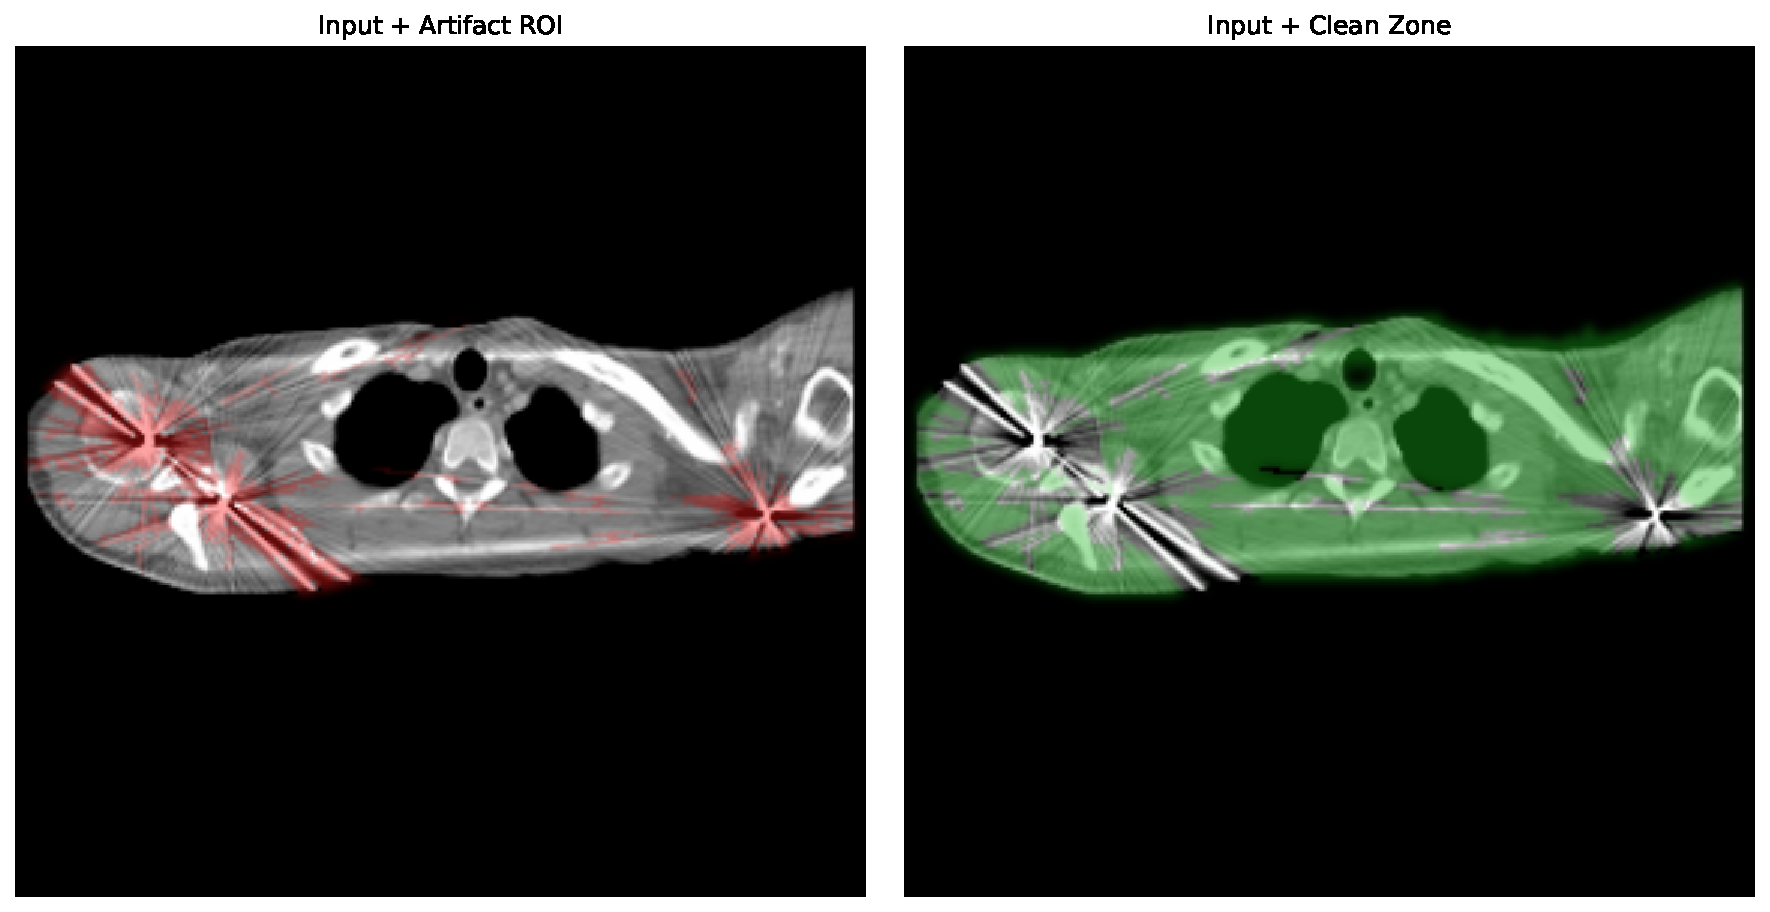
\includegraphics[width=0.95\linewidth]{Figures/roi_example_sample_0000.pdf}
\end{figure}

\begin{figure}[H]
    \centering
    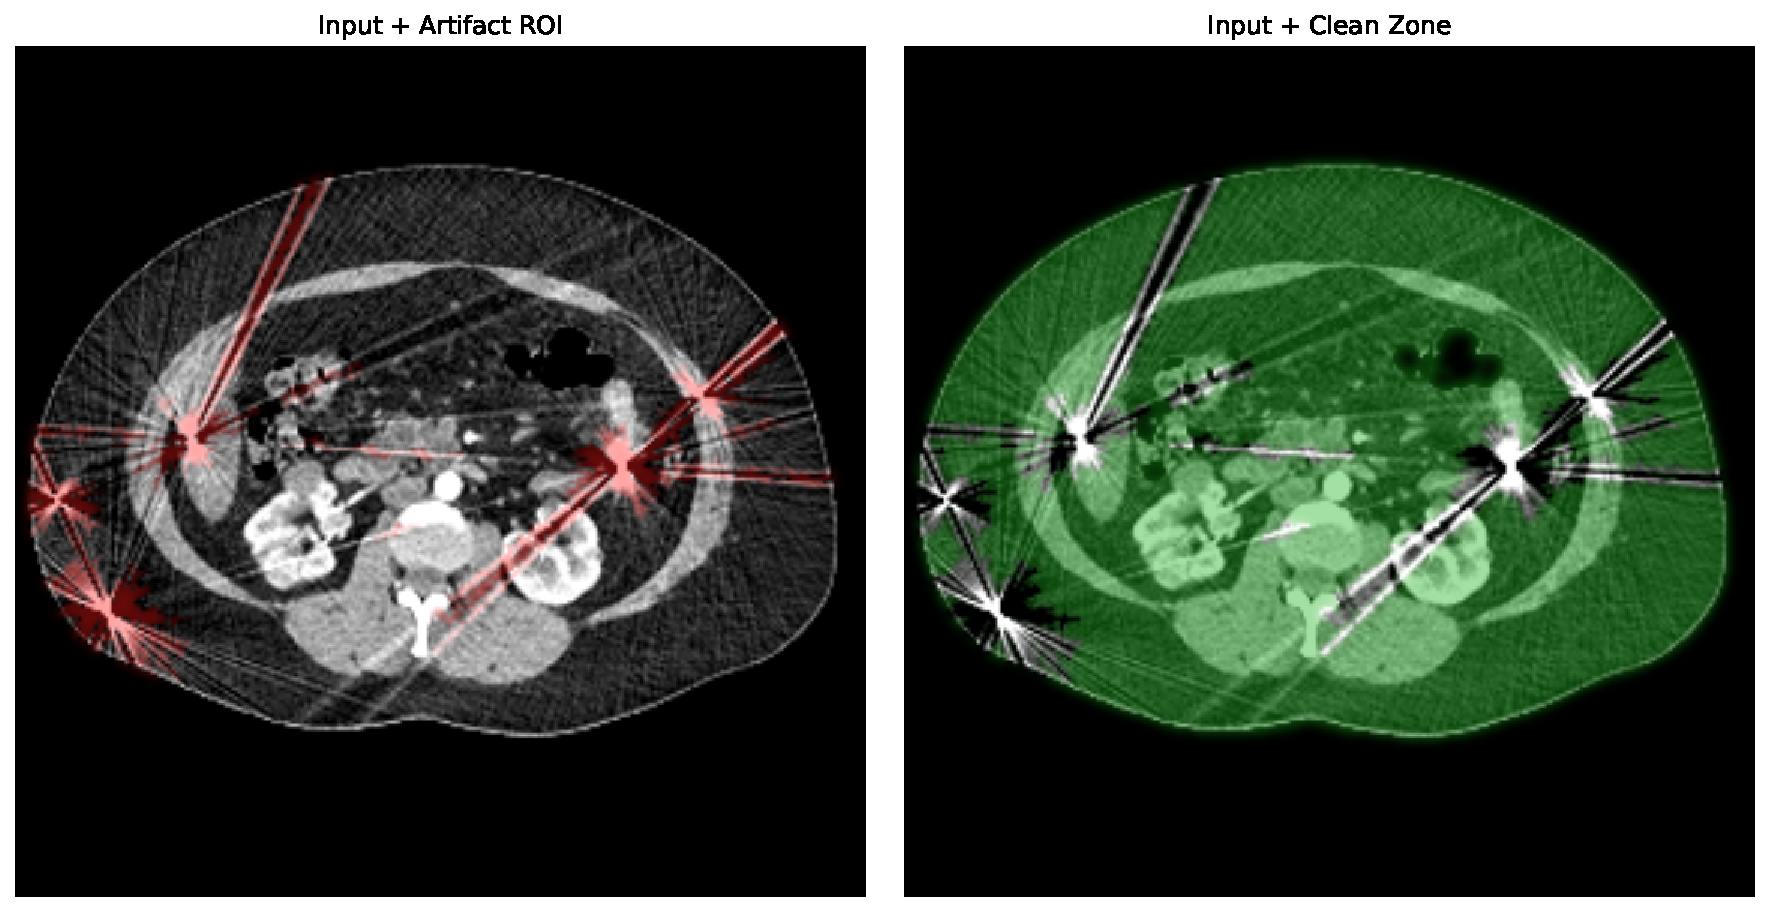
\includegraphics[width=0.95\linewidth]{Figures/roi_example_sample_0003.pdf}
\end{figure}

\begin{figure}[H]
    \centering
    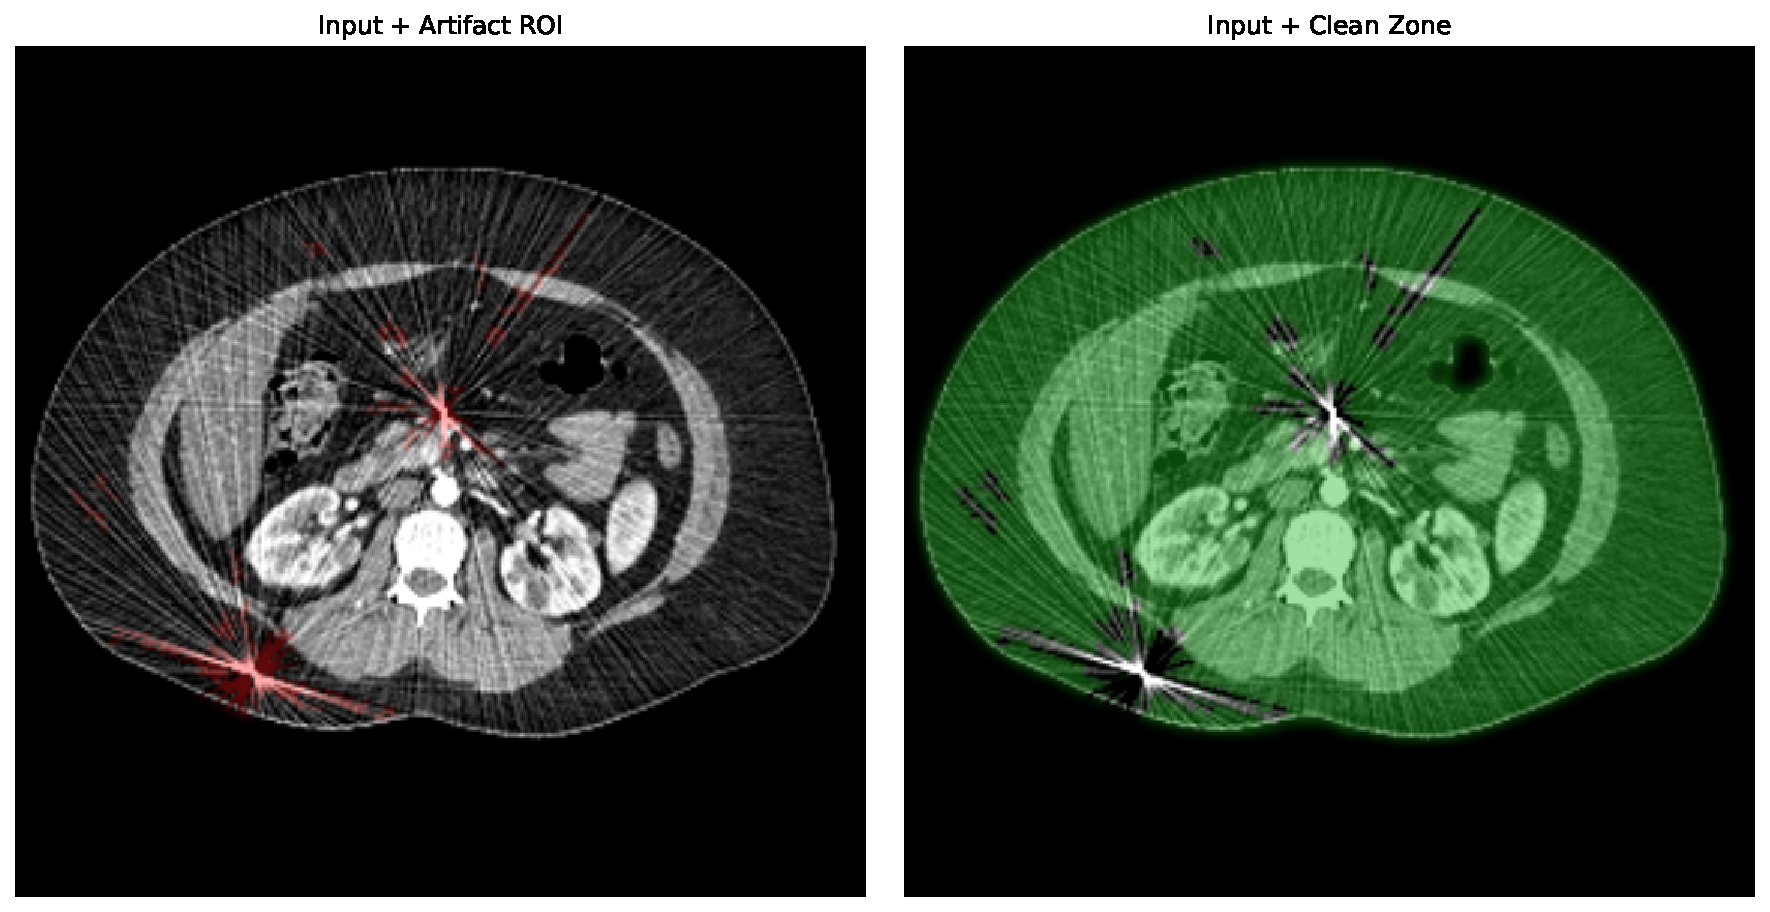
\includegraphics[width=0.95\linewidth]{Figures/roi_example_sample_0006.pdf}
\captionsetup{skip=1.5pt}
\caption[Artifact and clean ROI examples]{Artifact Zone\acrshort{roi} (left) and Clean Zone\acrshort{roi} (right) examples.}
\end{figure}
\label{fig:final-roi-examples}
\endgroup

In every evaluation context, the metrics were expressed as variations relative to the performance of the corrupted input. Global metrics was calculated too, as a complementary resource. Then, let $\Omega$ be the evaluation domain, which can correspond to the global region defined in the next subsection ($\Omega_{\mathrm{ Global}}$), the Artifact Zone ($\mathcal{R}_{\mathrm{ Art}}$), or the Clean Zone ($\mathcal{R}_{\mathrm{ Clean}}$), and let $\hat I$ be the reconstruction produced by the model. The variations were defined by:
\[
\Delta\mathrm{PSNR}_{\Omega} = \mathrm{PSNR}(\hat I\mid_{\Omega},\, I_{\mathrm{ref}}\mid_{\Omega}) - \mathrm{PSNR}(I_{\mathrm{in}}\mid_{\Omega},\, I_{\mathrm{ref}}\mid_{\Omega})
\]

\[
\Delta\mathrm{SSIM}_{\Omega} = \mathrm{SSIM}(\hat I\mid_{\Omega},\, I_{\mathrm{ref}}\mid_{\Omega}) - \mathrm{SSIM}(I_{\mathrm{in}}\mid_{\Omega},\, I_{\mathrm{ref}}\mid_{\Omega})
\]

\[
\Delta\mathrm{MAE}_{\Omega} = \mathrm{MAE}(I_{\mathrm{in}}\mid_{\Omega},\, I_{\mathrm{ref}}\mid_{\Omega}) - \mathrm{MAE}(\hat I\mid_{\Omega},\, I_{\mathrm{ref}}\mid_{\Omega}).
\]

Thus, $\Delta\mathrm{PSNR}>0$ and $\Delta\mathrm{SSIM}>0$ indicate improvement over the corrupted input. Since lower\acrshort{mae} represents better fidelity, the order of subtraction was reversed for this metric: $\Delta\mathrm{MAE}>0$ indicates error reduction and, therefore, improvement; $\Delta\mathrm{MAE}<0$ indicates error increase. Regular\acrshort{ssim} was used, calculated with a local window of $11\times11$ pixels and cropping with context around the evaluated region.

\begin{table}[H]
    \centering
    \begin{tabular}{lcccc}
        \hline
        \textbf{Metric} & \textbf{Train} & \textbf{Global} & \textbf{Artifact Zone} & \textbf{Clean Zone} \\
        \hline
        PSNR    & \checkmark & \checkmark & \checkmark & \checkmark \\
        SSIM    & \checkmark & \checkmark & \checkmark & \checkmark \\
        MAE     & \checkmark & \checkmark & \checkmark & \checkmark\\
        \hline
    \end{tabular}
    \caption[Evaluation metrics by context]{Evaluation metrics by context.}
    \label{tab:final-metrics-context}
\end{table}
%______________________________________________________________________________
\subsection{Global Metrics}
 After denormalization, the global evaluation region is cropped to the smallest bounding box of the body mask before\acrshort{ssim} evaluation, eliminating scan windows composed exclusively of background — which would artificially score $\text{SSIM} = 1{,}0$ and inflate the global metric.  

As an additional, purely descriptive check for any overall shift in average HU values, a Bland--Altman plot was made comparing the reconstruction with the clean reference. For each patient, the mean\acrshort{hu} of each image was calculated over all valid pixels of the body mask of the respective slices, weighted by the number of pixels in each slice. The graph plots the mean difference per patient ($\mathrm{Model}-\mathrm{GT}$) against the average of the two measurements, together with the average difference (bias) and the range within which most differences fall ($\bar d \pm 1{,}96\,SD_d$, the limits of agreement). This plot is descriptive only, one point per patient, and does not replace the accuracy metrics above or the region-based analysis above.

\subsection{Statistical Analysis}
Every statistical comparison in this work used the patient, not the slice, as the unit of analysis. A patient with more slices should not count more than a patient with fewer slices, so before any comparison, the per-slice metrics were averaged within each patient, giving one paired value per patient.

To evaluate the improvement over the corrupted input, for each patient the output's value was compared with the corrupted input's value, for both\acrshort{psnr} and\acrshort{ssim}, so that a positive difference always represents improvement. For\acrshort{mae}, whose reduction represents better performance, the subtraction was reversed so that a positive difference also represents improvement. In every test, the question asked was whether there was typically no difference at all between the paired values. The direct comparison between the two architectures followed the same logic, subtracting the Single Model's value from the Dual Model's value for each patient, so that negative differences favor the Single Model.

The $p$-values presented in the comparison tables were adjusted using the Holm sequential procedure, which controls the probability of at least one false positive across a family of related tests without assuming that the tests are independent: the smallest raw $p$-values are penalized the most, while the relative ordering between tests is preserved. This correction was computed in Python with the \texttt{multipletests} function from the \texttt{statsmodels} library, using the \texttt{'holm'} method.

In the reconstruction improvement table, the correction was applied jointly to the four corresponding tests for\acrshort{psnr} and\acrshort{ssim} for each of the two architectures. In the paired comparison Single Model vs Dual Model, the correction was applied jointly to the two tests, one for\acrshort{psnr} and another for\acrshort{ssim}.

The confidence interval of 95\% reported for the mean differences was obtained by patient-level percentile \textit{bootstrap}. For each metric, the vector of $n=41$ paired differences per patient was resampled with replacement, maintaining $n$ observations in each resample. The mean difference was then calculated in each of the 10,000 resamples. The lower and upper limits of the interval correspond, respectively, to the 2.5 and 97.5 percentiles of the empirical distribution of these means. This procedure does not assume normality of the differences and preserves the patient, rather than the slice, as the unit of inference. Seed 1337 was used to make the resampling deterministic.

\section{External Evaluation}
\label{sec:avaliacao-medicos}

The external evaluation was realized in independent data provided by the\acrfull{tcia} \cite{clarkCancerImagingArchive2013}, allowing to assess the impact of domain shift and the robustness of the model in scenarios not seen during training.

\subsection{Design and Cases}

The study consists in putting doctors to analyse the images produced by the model compared to the original images with artifacts. Every doctor looks at the same set of cases, one at a time, and for each one says which of the two images they prefer on a few simple questions. The evaluation was designed to be blind, with the doctors not knowing which image is the original and which is the model output. It was used a set of 15 samples from diverse\acrshort{tcia} datasets, with 2 additional hidden samples repeated for consistency check and 2 training samples excluded from the analysis. The 2 hidden repeats were shown again later in the same session, at least five cases after they first appeared, without telling the reader that it was a repeat.

A web application was developed to present the images in a randomized and counterbalanced manner, allowing the doctors to zoom jointly the pair for better visualization, and enabling two anatomical windowing options (soft tissue and lung). Whether the original or the model output appeared on the left or the right was shuffled between doctors, but kept the same when a case was repeated, so that this choice could not by itself explain any preference.

The link to the application was sent to the physicians invited by the researcher, rather than through an open call, with a target of seven participants and at least five required for the results to be useful. To take part, a doctor only had to confirm that they use\acrshort{ct} in their clinical practice at least once a month. No name, contact details, professional license number, or other proof of qualification was collected. The only information kept about each doctor is their country, medical specialty, how often they use CT, years of experience, previous experience with artifact reduction, and monitor type — none of which can identify a specific person.

The cases used in this evaluation were chosen from a larger pool of 48\acrshort{tcia} exams, mostly from the chest (31 cases), with a smaller number from the abdomen (6), the pelvis (1), and other or mixed regions (10). Each case corresponds to a single axial CT slice. The 17 cases used (15 main and 2 training) were drawn from five\acrshort{tcia} collections: TCGA-LUAD \cite{albertinaCancerGenomeAtlas2016}, LIDC-IDRI \cite{armatoDataLIDCIDRI2015}, VAREPOP-APOLLO \cite{repopVAResearchPrecision2024}, CPTAC-SAR \cite{cptacClinicalProteomicTumorSarcomas2019}, and CPTAC-PDA \cite{cptacClinicalProteomicTumorPancreatic2018}. 

In accordance with the data-usage policy of each collection, this work acknowledges: the results shown here are in whole or in part based upon data generated by the TCGA Research Network (\url{http://cancergenome.nih.gov/}), used in the TCGA-LUAD cases; the National Cancer Institute and the Foundation for the National Institutes of Health, for their critical role in the creation of the free publicly available LIDC/IDRI Database used in the LIDC-IDRI cases; the Veterans Health Administration's Research for Precision Oncology Program and the Applied Proteogenomics Organizational Learning and Outcomes (APOLLO) Research Network, whose data were used in the VAREPOP-APOLLO cases; and the National Cancer Institute Clinical Proteomic Tumor Analysis Consortium (CPTAC), whose data were used in the CPTAC-SAR and CPTAC-PDA cases.

\subsection{Quantitative Characterization of Input--Output}

As a complementary characterization of the alteration introduced by the model in external cases,\acrshort{ssim},\acrshort{psnr}, and\acrshort{mae} were calculated directly between the input image and the respective output of the model selected for that. The metrics was evaluated only in the 15 main cases of the frozen external set. The two training cases were excluded. The calculation domain was the effective body mask, manually corrected during case preparation. For\acrshort{psnr}, the intensity window $[-1000,400]$\acrshort{hu} with amplitude $1400$\acrshort{hu} was used.

There is no clean reference for these real cases. Thus, higher\acrshort{ssim} and\acrshort{psnr}, as well as lower\acrshort{mae}, describe less global alteration between input and output, and not greater accuracy of artifact removal or improvement compared to a reference. The statistics were summarized per case, such as mean and standard deviation, and the 95\% confidence intervals for the mean were obtained by percentile \textit{bootstrap} with 10,000 resamplings and seed 1337. The interpretation of the clinical acceptability of these alterations remained reserved for blind evaluation by readers.

\subsection{Presentation and Evaluation Instrument}

For each case, the two images, the artifact input and the model output, are shown side by side at the same time, labelled only ``Image A'' and ``Image B'', with nothing on screen indicating which is which. After looking at a case, the doctor answers four short questions, always with the same three possible answers: ``Image A'', ``Image B'', or ``No difference''. In turn, these questions ask which image has less visible metal artifact, which image better shows the anatomy hidden behind the artifact (this is the main question of the study), which image has fewer artifacts or distortions in the rest of the picture, away from the artifact, and which image the doctor would prefer to use for a clinical read. The third question exists specifically to catch a possible unwanted effect of the model: if doctors tend to prefer the artifact input in regions away from the implant, that would suggest the model is introducing changes where none were needed. At the very end of the session, each doctor answers one extra question, on a five-point scale from ``Definitely not'' to ``Definitely yes'', about whether a processed version like this could be a useful addition to a normal\acrshort{ct} exam, and may optionally leave a short written comment.

\subsection{Outcomes and Analysis}

The main question of the study, the primary outcome, is which image better shows the anatomy under the metal artifact, taken from the corresponding question described above. Each displayed A/B answer was recoded to input, output, or no difference using the saved left/right allocation. To account for the fact that every reader judged every case, response proportions and the primary output--input contrast were accompanied by 95\% percentile confidence intervals from a two-way non-parametric cluster bootstrap, resampling readers and cases independently (10,000 resamples; seed 2024). The other three per-case questions, together with the final usefulness question, are treated as secondary outcomes and are summarized using the same descriptive approach; no multiplicity correction was applied.

Because two cases are shown a second time to each doctor later in the same session, without saying so, it is possible to check how consistent each doctor is with themselves. As these are nominal three-category responses and only two repeat pairs are available per reader, consistency is reported descriptively as exact agreement between the original and repeated answer for each question. Given the small number of doctors expected to take part, the confidence intervals and repeat agreement are interpreted descriptively rather than as definitive clinical evidence.

\subsection{Operational Status}

Before any real doctor took part, the application was first tested with a technical pilot using placeholder data, to check that the questions, the images, and the randomization all worked as intended. Moving from this rehearsal stage to inviting real doctors was only allowed once a documented checklist was fully satisfied, covering an approved and tested hosting setup, a defined data retention and deletion plan, an approved participant information text, and a working, secure deployment of the application.
